\begin{figure}[p]
\centering
    \begin{subfigure}[t]{\textwidth}
        \centering
    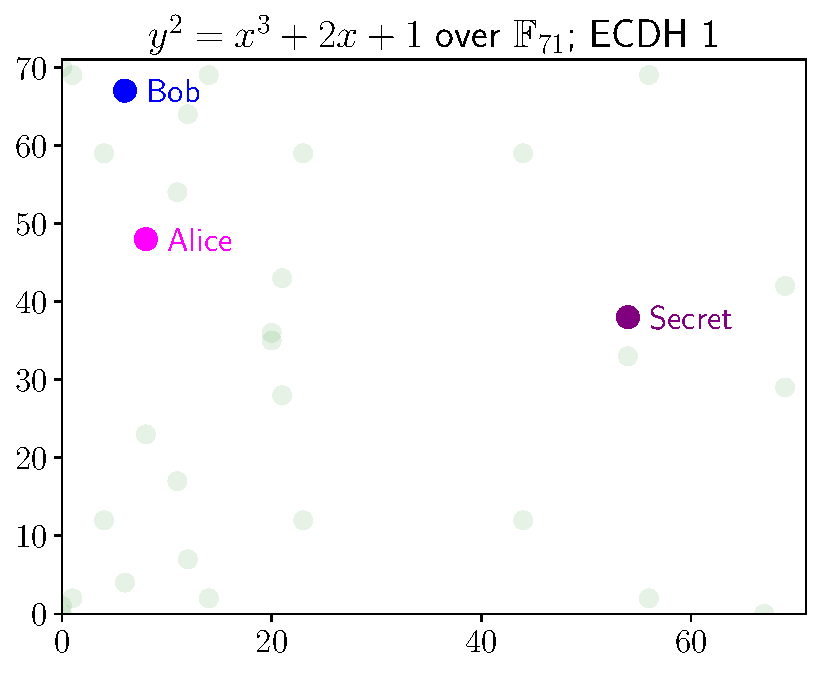
\includegraphics[width=0.70\textwidth]{plots/ec_finite/ec_finite_F_71_2_1_ecdh_1.pdf}
    \caption{Plot of Alice's public key ${\color{magenta}{A}} = \parens{8,48}$,
    Bob's public key ${\color{blue}{B}} = \parens{6,67}$,
    and the \gls{shared secret} ${\color{purple}{K}} = \parens{54,38}$
    for Example~\ref{example:ecc_ecdh_1}.}
    \label{fig:ec_finite_plots_ecdh_1}
    \end{subfigure}

    \begin{subfigure}[t]{\textwidth}
        \centering
    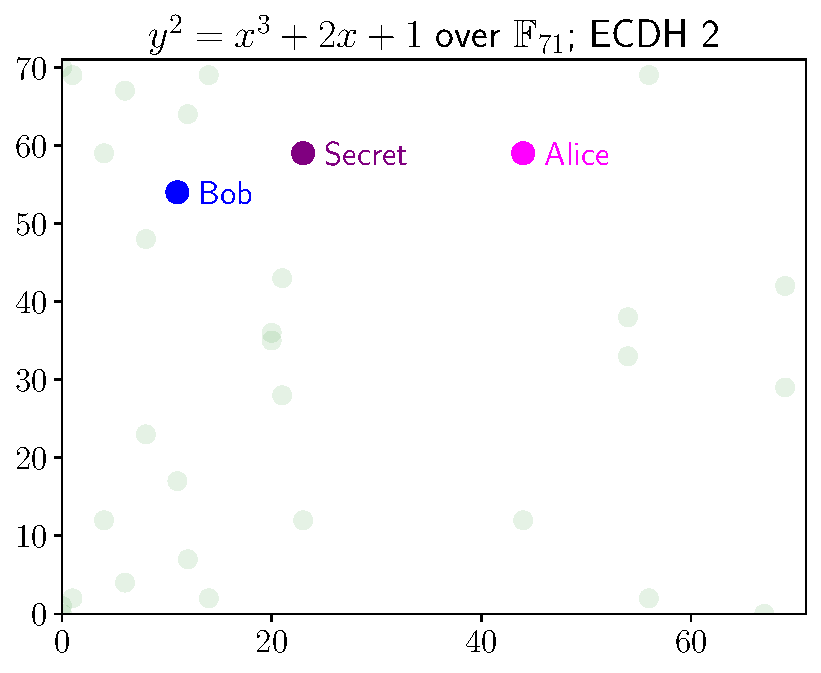
\includegraphics[width=0.70\textwidth]{plots/ec_finite/ec_finite_F_71_2_1_ecdh_2.pdf}
    \caption{Plot of Alice's public key ${\color{magenta}{A}} = \parens{44,59}$,
    Bob's public key ${\color{blue}{B}} = \parens{11,54}$,
    and the \gls{shared secret} ${\color{purple}{K}} = \parens{23,59}$
    for Example~\ref{example:ecc_ecdh_2}.}
    \label{fig:ec_finite_plots_ecdh_2}
    \end{subfigure}

\caption[Plots of public keys and shared secrets for ECDH]{Here
    we plot Alice's public key ${\color{magenta}{A}} = a\cdot P$,
    Bob's public key ${\color{blue}{B}} = b\cdot P$,
    and the \gls{shared secret} ${\color{purple}{K}} = (ab)\cdot P$
    for Examples~\ref{example:ecc_ecdh_1} and \ref{example:ecc_ecdh_2}.
    }
\label{fig:ec_finite_plots_ecdh}
\end{figure}
